\documentclass{article}
\usepackage{v-equation}
\vgeometry

\begin{document}

\def\gdrive{https://drive.google.com/drive/folders/1dkPrQ_j6XT03l7yuzVTc3xlHoBMPhdXs?usp=share_link}
\vtitle[\texttt{Conjugate Complex Number}]

\begin{center}
\begin{tikzpicture}
	\tzaxes(-1, -3)(4,3){\textit{Real axis}}{\textit{Imaginary axis}}
	\tzcoor*(3, 2)(Z){$z$}[r]
	\tzcoor*(3, -2)(Z'){$\overline{z}$}[r]
	\tzline[->](0, 0)(Z)
	\tzline[->](0, 0)(Z')
	%\tzline[|<->|]<0, -0.5>(0, 0)(3, 0){$a$}[mb]
	%\tzline[|<->|]<-0.5, 0>(0, 0)(0, 2){$b$}[ml]
	\tzanglemark(3, 0)(0, 0)(Z){$\theta$}(15pt)
	\tzanglemark'(3, 0)(0, 0)(Z'){$\theta$}(15pt)
\end{tikzpicture}
\end{center}
\vspace*{\fill}
\addtolength{\jot}{3ex}
\begin{align*}
z &= a + ib \\
\overline{z} &= a - ib
\end{align*}
\vspace*{\fill}

\pagebreak

\vspace*{\fill}
\begin{center}
    \fbox{\qrcode[height=2cm]{\gdrive}}
\end{center}
\vspace*{\fill}
\end{document}
